% Exercise ID: MAT_P4FUNCOE_4FIN_GRA_004
% Exercise ID: MAT_P4FUNCOE_4FIN_GRA_004
% Module: MÓDULO P4 - Funções | Concept: Função Inversa | Type: Determinação Gráfica
% Difficulty: 2/5 (Fácil) | Type: desenvolvimento
% Points: 10 | Time: 10 min
% Tags: inversa, grafico, simetria, funcao_quadratica
% Author: Professor | Date: 2025-11-18
% Status: active
% Description: Dado o gráfico de ramos de funções, desenhar o gráfico da inversa

\exercicio
Na figura está representado o gráfico de uma função $f$ definida em $[1, 4]$. Represente, no referencial dado, o gráfico da função inversa $f^{-1}$.

\begin{figure}[ht]
\centering
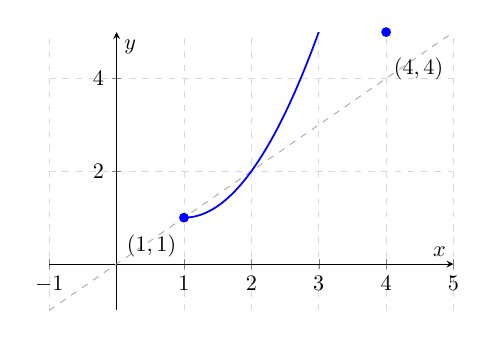
\begin{tikzpicture}[scale=0.8]
    \begin{axis}[
        axis lines = middle,
        xlabel = $x$,
        ylabel = $y$,
        xmin = -1, xmax = 5,
        ymin = -1, ymax = 5,
        grid = major,
        grid style = {dashed, gray!30},
        width = 8cm,
        height = 6cm,
    ]
    \addplot[domain=-1:5, dashed, gray!70, thin] {x};
    
    \addplot[domain=1:4, samples=100, thick, blue] {(x-1)^2 + 1};
    \addplot[mark=*, mark size=2pt, blue] coordinates {(1,1)};
    \addplot[mark=*, mark size=2pt, blue] coordinates {(4,10/2)};
    \node[anchor=west] at (axis cs:4,4.2) {$(4,4)$};
    \node[anchor=north east] at (axis cs:1,0.8) {$(1,1)$};
    \end{axis}
\end{tikzpicture}
\end{figure}

\bigskip

\exercicio
Na figura está representado o gráfico de uma função $g$ definida em $]0, 4]$. Represente, no referencial dado, o gráfico da função inversa $g^{-1}$.

\begin{figure}[H]
\centering
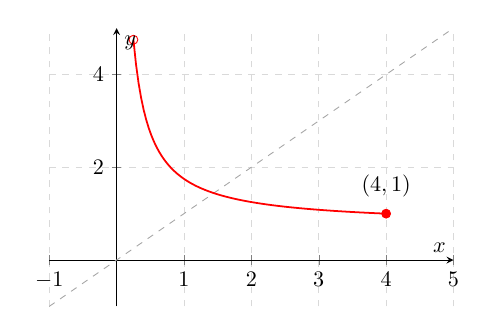
\begin{tikzpicture}[scale=0.8]
    \begin{axis}[
        axis lines = middle,
        xlabel = $x$,
        ylabel = $y$,
        xmin = -1, xmax = 5,
        ymin = -1, ymax = 5,
        grid = major,
        grid style = {dashed, gray!30},
        width = 8cm,
        height = 6cm,
    ]
    \addplot[domain=-1:5, dashed, gray!70, thin] {x};
    
    \addplot[domain=0.25:4, samples=100, thick, red] {1/x + 0.75};
    \addplot[mark=o, mark size=2pt, red] coordinates {(0.25,4.75)};
    \addplot[mark=*, mark size=2pt, red] coordinates {(4,1)};
    \node[anchor=south] at (axis cs:4,1.2) {$(4,1)$};
    \end{axis}
\end{tikzpicture}
\end{figure
\vspace{3cm}
}
